\documentclass[al, 27pt, plainboxedsections, landscape]{sciposter}
\usepackage{multicol}
\usepackage{sectionbox}
\usepackage[demo]{graphicx}
\usepackage{subfig}
\usepackage[numbers, longnamesfirst, sort]{natbib}

\definecolor{darkgreen}{rgb}{0,0.4,0}

\newcommand{\tb}[1]{\textcolor{blue}{#1}}
\newcommand{\tre}[1]{\textcolor{red}{#1}}
\newcommand{\tgrey}[1]{\textcolor{grey}{#1}}
\newcommand{\tgr}[1]{\textcolor{darkgreen}{#1}}
\newcommand{\tye}[1]{\textcolor{yellow}{#1}}
\newcommand{\cya}[1]{\textcolor{cyan}{#1}}
\newcommand{\cnt}[1]{{\tt \textcolor{cyan}{#1}}}

\title{Computing Kantorovich-Wasserstein Distances on $d$-dimensional histograms using $(d+1)-$partite graphs}
\leftlogo[1.3]{images/logo_unipv}

\author{Gennaro Auricchio$^{a}$, Federico Bassetti$^b$, Stefano Gualandi$^a$, Marco Veneroni$^a$}
\institute{$^{(a)}$ Universit\`{a} degli Studi di Pavia, Dipartimento di Matematica ``F.Casorati'',$\quad ^{(b)}$ Politecnico di Milano, Dipartimento di Ingegneria Matematica}
\email{gennaro.auricchio01@universitadipavia.it,stefano.gualandi@unipv.it,marco.veneroni@unipv.it,federico.bassetti@polimi.it}

\begin{document}
\maketitle
\begin{multicols}{3}
	
	\begin{abstract}	
	\large{	
		\begin{itemize}		
			\item[] \tgr{{\bf TASK}: To compute the distance between two $d$-dimensional histograms having $n$ bins. For instance, images are 2-dimensional histograms with $n$ bins (pixels)}
			\item[] \tb{{\bf PROBLEM}: The mathematical tool used to compute this distance requires the solution of an optimization problem with up to $n^2$ variables}
			\item[] \tre{{\bf IDEA}: To exploit the structure of the cost function in order to reduce the number of variables of the optimization problem}
		\end{itemize}}
	\end{abstract}
	
\section{Optimal Transport} 
 The optimal transport is a tool that is nowadays used to compute distances between images. For example the $W_2$ distance is used in image processing, but it is still a problem to compute $W_2$ efficiently. 

 \begin{figure}
     \centering
     {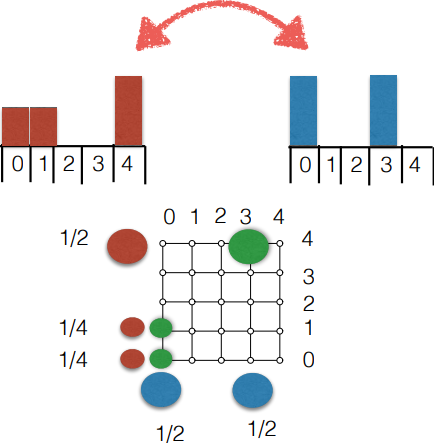
\includegraphics[width=0.35\columnwidth]{images/intro_disc}\label{<figure1>}}
	 \hspace{0.05\columnwidth}
     {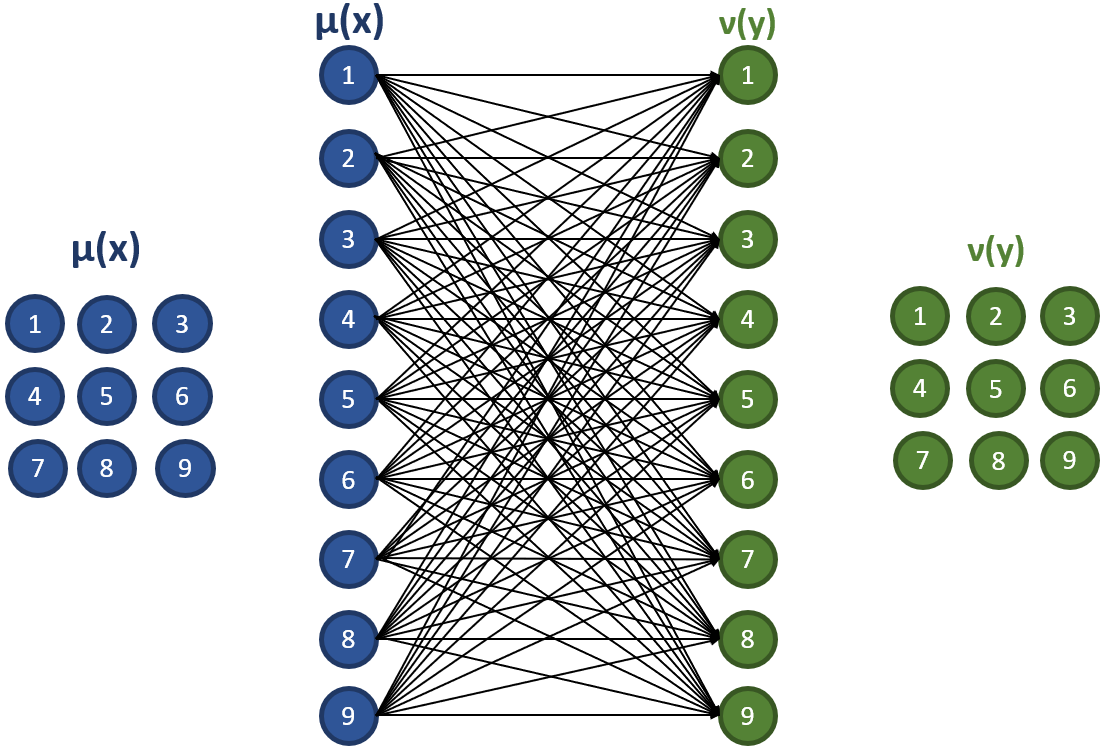
\includegraphics[width=0.45\columnwidth]{images/fig3}\label{<figure2>}}
     \caption{Left: Blablabla. Right: blablabla}
     \label{steady_state}
\end{figure}

 The problem outline is the following: given two different configurations, that we will represent with two probability measures, we want to rearrange one into the other one. 

For the sake of clarity and brevity we will work with $2D$ grids.\newline
	
We want to find the optimal way to map a probability $\mu$ to a probability $\nu$ where moving a unit mass from $x$ to $y$ costs $c(x, y)=(x_1-y_1)^2 + (x_2-y_2)^2$, so we consider
\[
W_2(\mu,\nu) := \min \sum_{x \in X}\sum_{y\in Y}c(x,y) \pi_{x,y}
\]
where the minimum is taken over all the probability measures $\pi_{x,y}$ such that
\[
\sum_{x \in X}\pi_{x,y}=\nu_y, \;\;\;\;\; \emph{and}  \;\;\;\;\; \sum_{y \in Y}\pi_{x,y}= \mu_x.
\]

This can be done only for some images (we can compute this quantity only when they have equal mass), but actually it can applied to each image, also to histograms, if we normalize them. 


\section{Our Reformulation}
The standard approach to compute $W_2$ distances between $2D$ histograms with $n = N^2$ bins can be seen as an Uncapacitated Min Cost Flow problem on a bipartite graph, with $2n$ nodes and $n^2$ arcs, and can then be solved in $O(n^3 \log (n))$ time.\newline

Those huge numbers are due to the large amount of connections we need, as showed in the following figure.

\begin{figure}[!t]
	\centering
	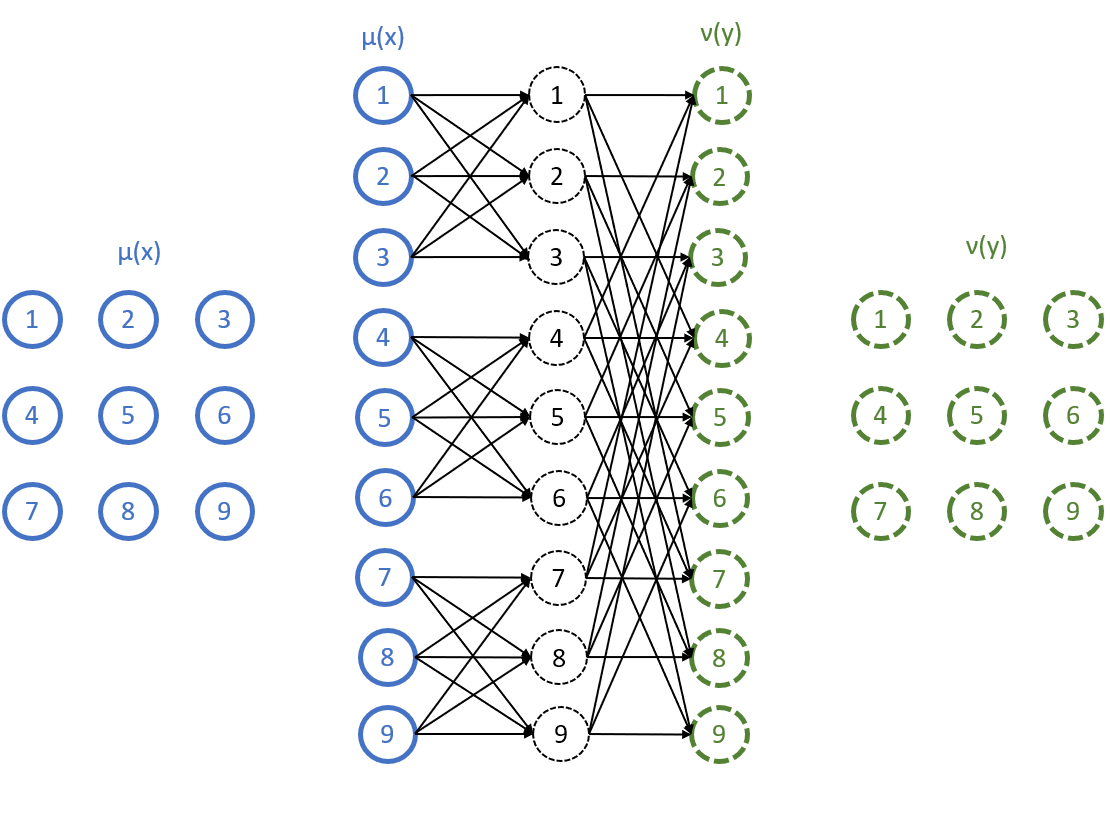
\includegraphics[width=0.55\columnwidth]{images/fig6}
\end{figure}

In our paper we present a novel approach to this computation that exploits the structure of the cost function to reduce the number of connections needed.\newline

In fact, since the cost function is the sum of two independent contributes, we can describe each transport from a generic point to another one as the concatenation of two transports along the two main directions.

As a consequence of this fact, we can show that the $W_2$ distance can be computed as a flux problem on a $3-$partite graph, as illustrated in the following picture.



In this way, rather than connect each bin to each bin, we effectuate two connections: the first one between each bin and each other bin aligned along the first main direction and the second one between bins aligned along the second main direction.\newline

This simple change of formulation reduces drastically the computational cost, but there is even more:
\begin{itemize}
	\item This reasoning is easily adaptable to grids of any dimension $d$ and the method escalates very well with it: while the old method required $n^2$ connections, this methods only requires $dn^{1+\frac{1}{d}}$.
	\item We can also adapt this method to each cost function that is separable, \emph{i.e.} can be written as sum of independent contributions.
	\item  As showed in the next section, this method outperforms all known approximated methods and still provides us the exact computation.
\end{itemize}


\section{Numerical Results}

\begin{table}
\caption{Comparison on Flow Cytometry data with increasing value of $d$.}
	\label{tab:3}
\centering
{\renewcommand{\arraystretch}{1.2}
\begin{tabular}{llrrrrrrr}
     & & & \multicolumn{3}{c}{Bipartite Graph} & \multicolumn{3}{c}{$(d+1)$-partite Graph} \\
N & $d$ & $n$ & $|V|$ & $|A|$ & Runtime & $|V|$ & $|A|$ & Runtime  \\
\hline
$16$ & 2 & 256 & 512 & 65\,536 & 0.024 (0.01) & 768 & 8\,192 & 0.003 (0.00) \\
& 3 & 4\,096 & 8\,192 & 16\,777\,216& 38.2 (14.0)   & 16\,384 & 196\,608& 0.12 (0.02)  \\
& 4 & 65\,536 & \multicolumn{3}{c}{{\it out-of-memory}} & 327\,680 & 4\,194\,304& 4.8 (0.84) \\
 \hline\noalign{\smallskip}
$32$ & 2 & 1\,024 & 2\,048 & 1\,048\,756 & 0.71 (0.14) & 3072 & 65\,536& 0.04 (0.01) \\
& 3 & 32\,768& \multicolumn{3}{c}{{\it out-of-memory}}   & 131\,072 & 3\,145\,728& 5.23 (0.69)  \\
 \hline\noalign{\smallskip}
 \end{tabular}}
\end{table}

\begin{figure}[!t]
\centering
{\renewcommand{\arraystretch}{0.7}
\setlength{\tabcolsep}{0.1em}
\begin{tabular}{cccccccccc}
  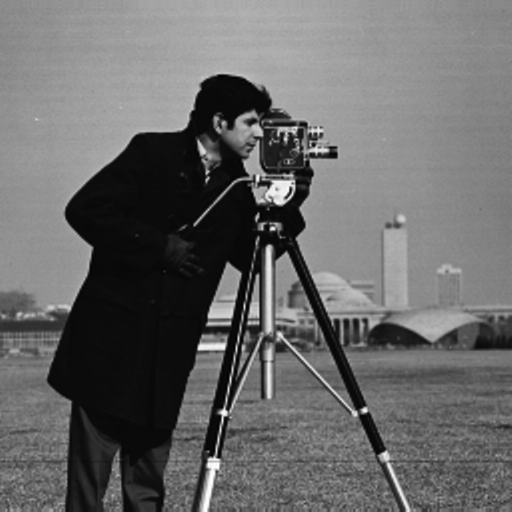
\includegraphics[width=0.095\linewidth]{images/classic512_1001}  & 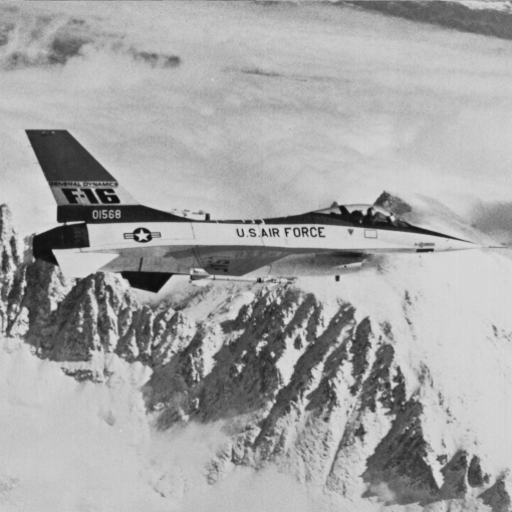
\includegraphics[width=0.095\linewidth]{images/classic512_1002} &
  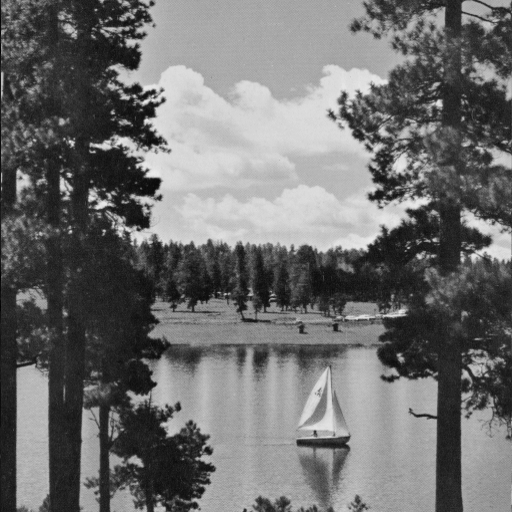
\includegraphics[width=0.095\linewidth]{images/classic512_1003} & 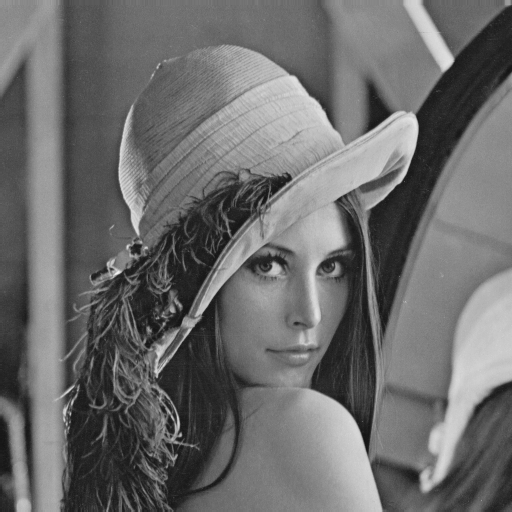
\includegraphics[width=0.095\linewidth]{images/classic512_1004} &
  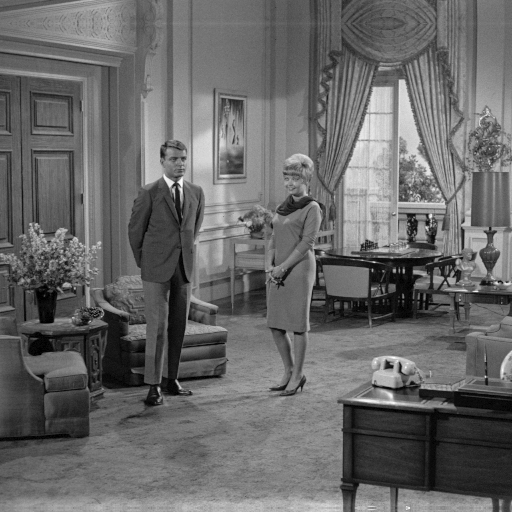
\includegraphics[width=0.095\linewidth]{images/classic512_1005} &
  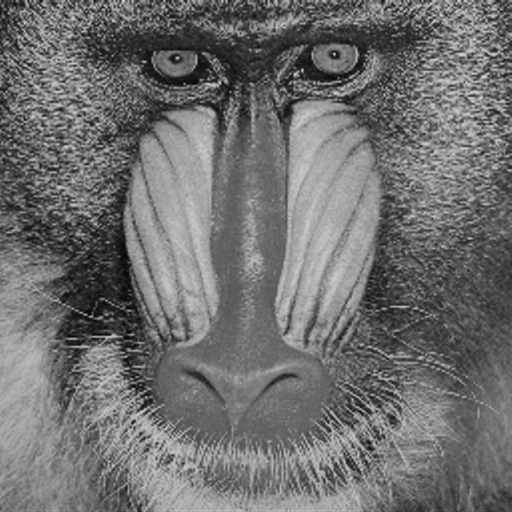
\includegraphics[width=0.095\linewidth]{images/classic512_1006}  & 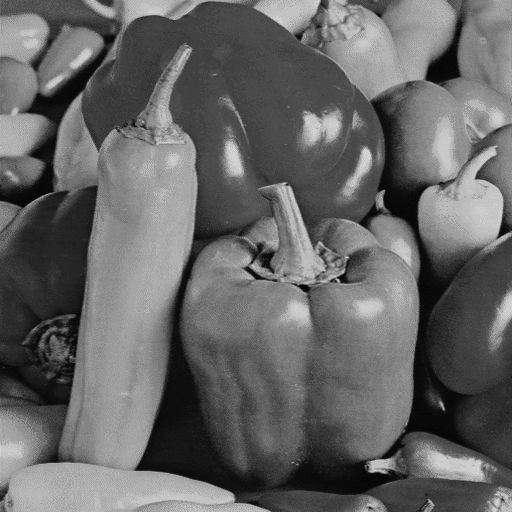
\includegraphics[width=0.095\linewidth]{images/classic512_1007} &
  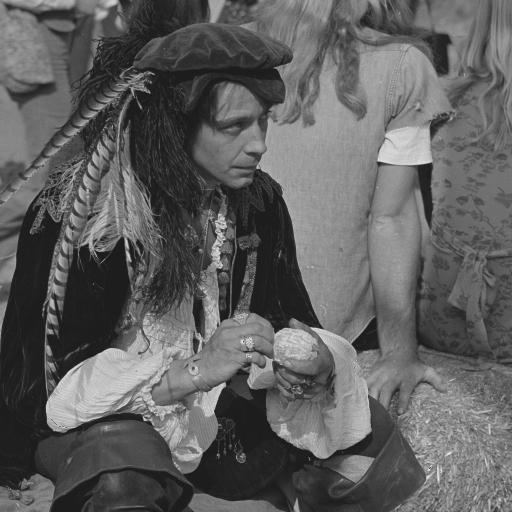
\includegraphics[width=0.095\linewidth]{images/classic512_1008} & 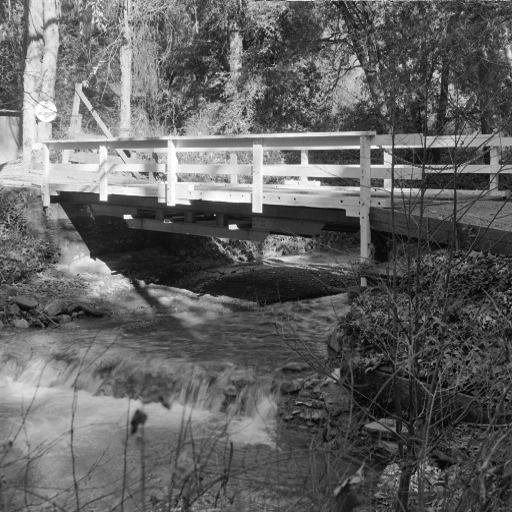
\includegraphics[width=0.095\linewidth]{images/classic512_1009} &
  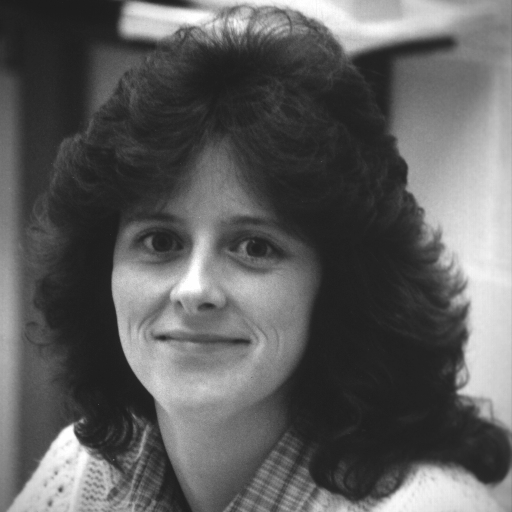
\includegraphics[width=0.095\linewidth]{images/classic512_1010} \\  
  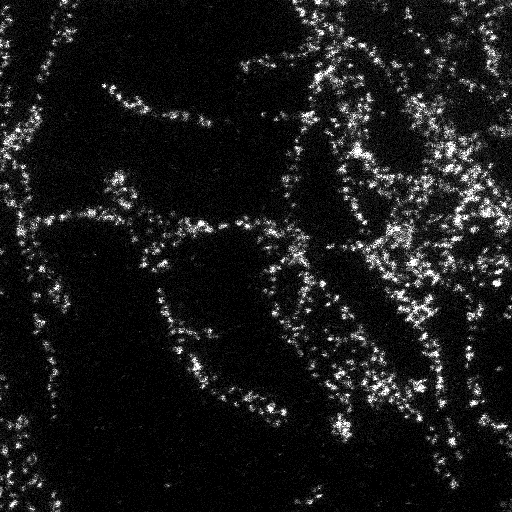
\includegraphics[width=0.095\linewidth]{images/micro512_1001}  & 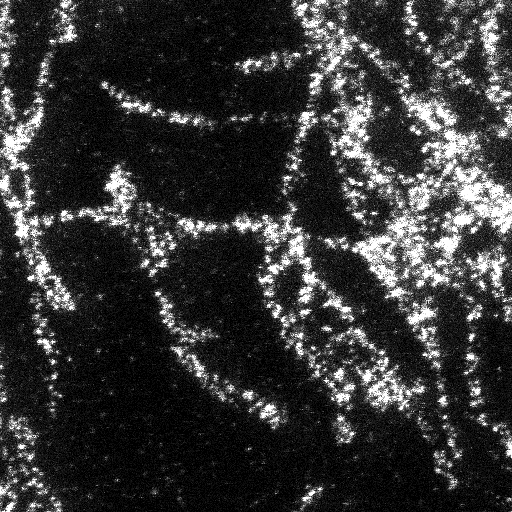
\includegraphics[width=0.095\linewidth]{images/micro512_1002} &
  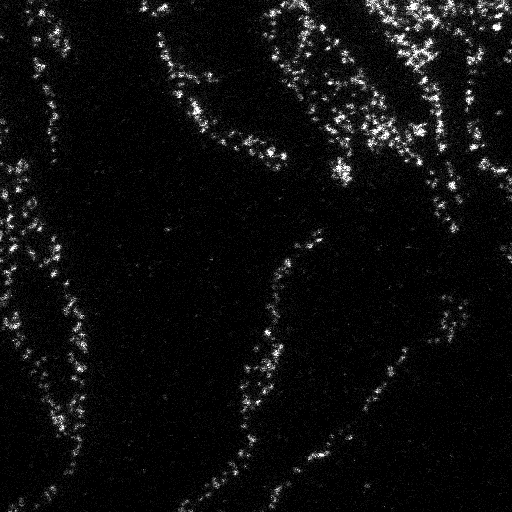
\includegraphics[width=0.095\linewidth]{images/micro512_1003} & 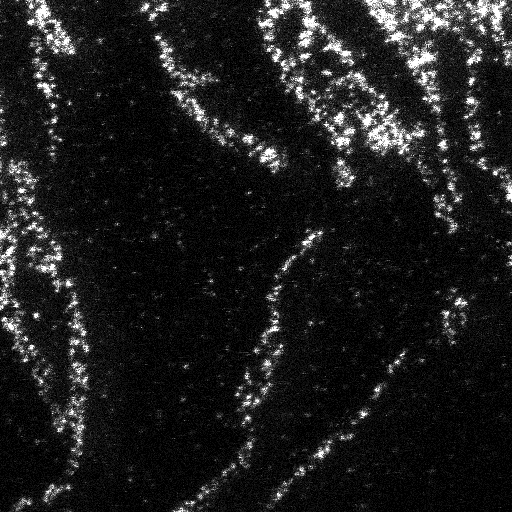
\includegraphics[width=0.095\linewidth]{images/micro512_1004} &
  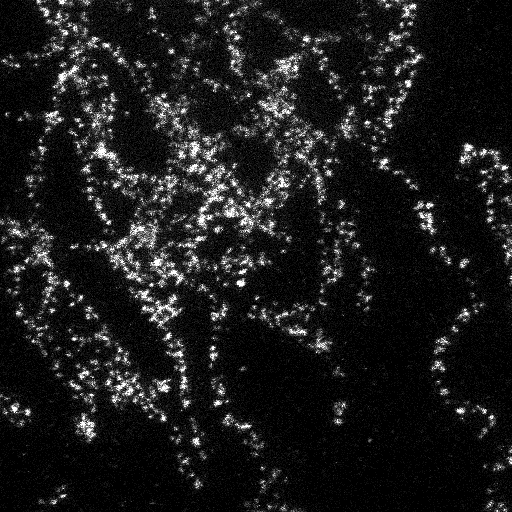
\includegraphics[width=0.095\linewidth]{images/micro512_1005} &
  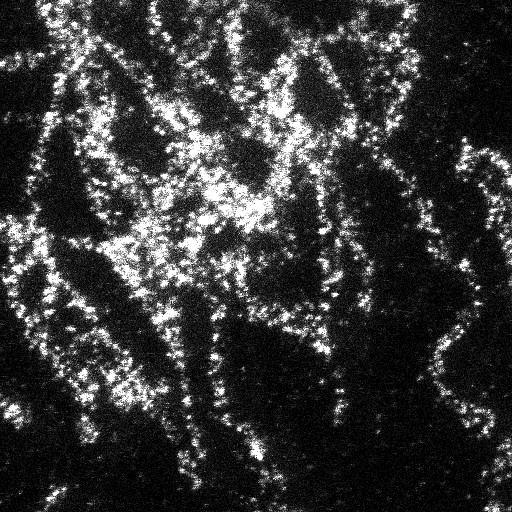
\includegraphics[width=0.095\linewidth]{images/micro512_1006}  & 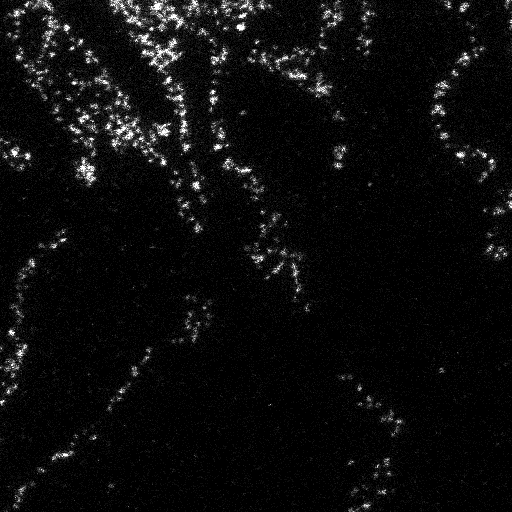
\includegraphics[width=0.095\linewidth]{images/micro512_1007} &
  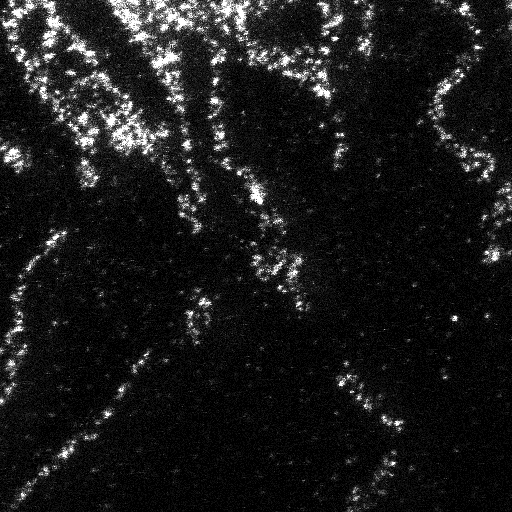
\includegraphics[width=0.095\linewidth]{images/micro512_1008} & 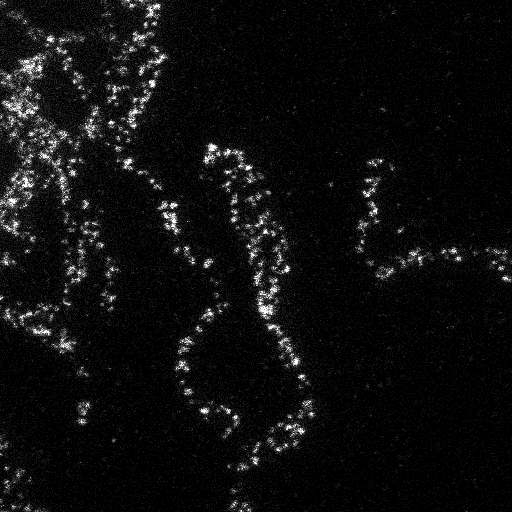
\includegraphics[width=0.095\linewidth]{images/micro512_1009} &
  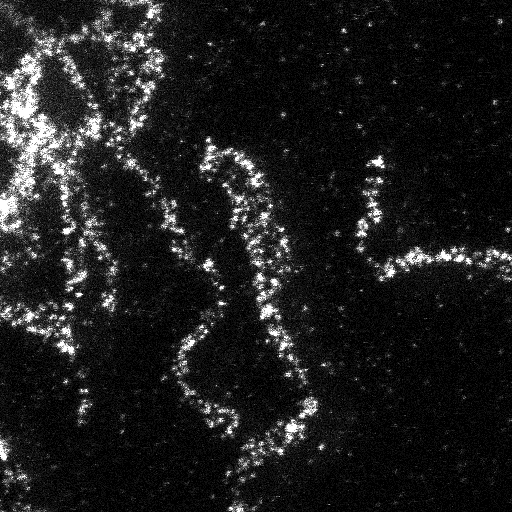
\includegraphics[width=0.095\linewidth]{images/micro512_1010} \\
    
\includegraphics[width=0.095\linewidth]{images/shapes512_1001}  & 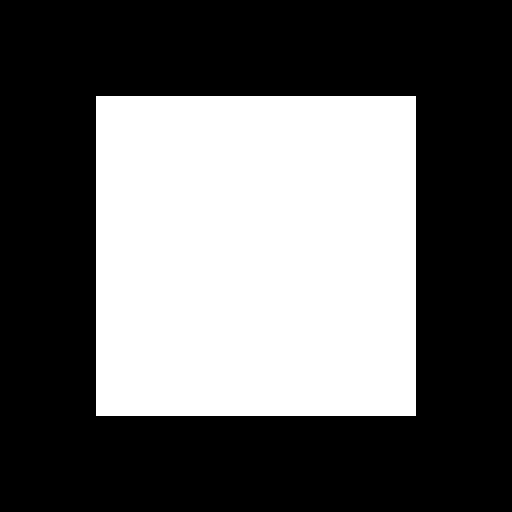
\includegraphics[width=0.095\linewidth]{images/shapes512_1002} &
  
\includegraphics[width=0.095\linewidth]{images/shapes512_1003} & 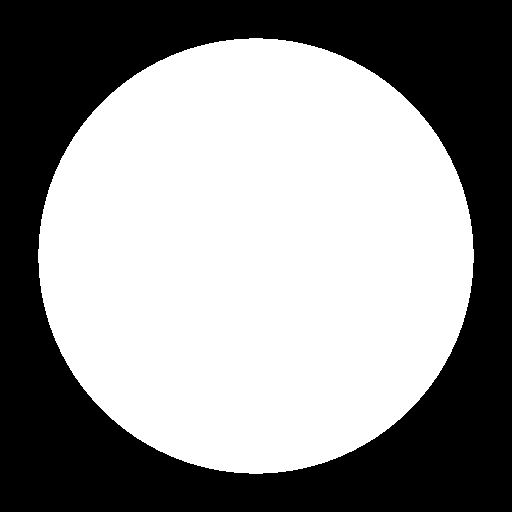
\includegraphics[width=0.095\linewidth]{images/shapes512_1004} &
  
\includegraphics[width=0.095\linewidth]{images/shapes512_1005} &
  
\includegraphics[width=0.095\linewidth]{images/shapes512_1006}  & 
\includegraphics[width=0.095\linewidth]{images/shapes512_1007} &
  
\includegraphics[width=0.095\linewidth]{images/shapes512_1008} & 
\includegraphics[width=0.095\linewidth]{images/shapes512_1009} &
  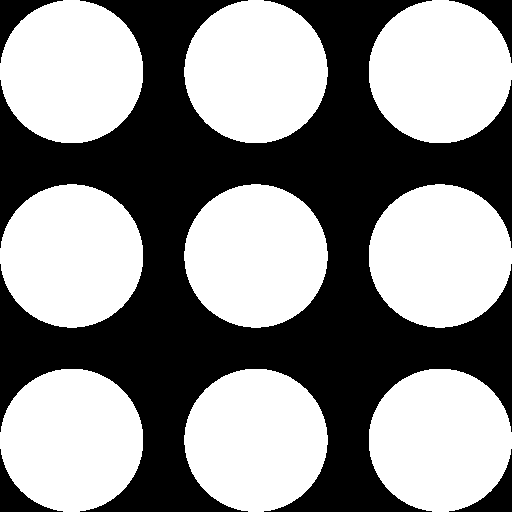
\includegraphics[width=0.095\linewidth]{images/shapes512_1010} \\
 \end{tabular}}
\caption{DOTmark benchmark: Classic, Microscopy, and Shapes images. \label{fig:dot}}
\end{figure}

\begin{table}[t!]
\caption{Comparison of different approaches on $32 \times 32$ images. The runtime (in seconds) is given as ``Mean (StdDev)''.
The gap to the optimal value {\it opt} is computed as $\frac{UB-opt}{opt}\cdot 100$, where $UB$ is the upper bound computed by Sinkhorn's algorithm.
Each row reports the averages over 45 instances.
\label{tab:1}}
\centering
{\renewcommand{\arraystretch}{1.2}
\begin{tabular}{lccrcrcc}
      & \multicolumn{1}{c}{EMD\cite{Rubner98}} &  \multicolumn{4}{c}{Sinkhorn \cite{Cuturi2013}} & \multicolumn{1}{c}{Bipartite} & \multicolumn{1}{c}{$3$-partite} \\
	  & & \multicolumn{2}{c}{$\lambda=1$} & \multicolumn{2}{c}{$\lambda=1.5$} &  &  \\
Image Class & Runtime & Runtime & Gap & Runtime & Gap & Runtime & Runtime \\
\hline
Classic    & 24.0 (3.3) & 6.0 (0.5) & 17.3\% & 8.9 (0.7) & 9.1\%  & 0.54 (0.05) & 0.07 (0.01)\\
Microscopy & 35.0 (3.3) & 3.5 (1.0) &  2.4\% & 5.3 (1.4) & 1.2\% & 0.55 (0.03) & 0.08 (0.01)\\
Shapes     & 25.2 (5.3) & 1.6 (1.1) &  5.6\% & 2.5 (1.6) & 3.0\% & 0.50 (0.07) & 0.05 (0.01)\\
 \hline\noalign{\smallskip}
 \multicolumn{8}{c}{} \\
 \end{tabular}}
\centering
{\renewcommand{\arraystretch}{1.2}
\setlength{\tabcolsep}{5pt}
\begin{tabular}{lcrcrcrc}
      & \multicolumn{6}{c}{Improved Sinkhorn \cite{Solomon2015,Solomon2018}} & \multicolumn{1}{c}{$3$-partite} \\
	  & \multicolumn{2}{c}{$\lambda=1$} & \multicolumn{2}{c}{$\lambda=1.25$}  & \multicolumn{2}{c}{$\lambda=1.5$}  &  \\
Image Class     & Runtime           & Gap       & Runtime           & Gap       & Runtime           & Gap       &   Runtime \\
\hline
 CauchyDensity	&	0.22	(0.15)	&	2.8\%	&	0.33	(0.23)	&	2.0\%	&	0.41	(0.28)	&	1.5\%	&	0.07	(0.01)	\\
 Classic		&	0.20	(0.01)	&	17.3\%	&	0.31	(0.02)	&	12.4\%	&	0.39	(0.03)	&	9.1\%	&	0.07	(0.01)	\\
 GRFmoderate	&	0.19	(0.01)	&	12.6\%	&	0.29	(0.02)	&	9.0\%	&	0.37	(0.03)	&	6.6\%	&	0.07	(0.01)	\\
 GRFrough		&	0.19	(0.01)	&	58.7\%	&	0.29	(0.01)	&	42.1\%	&	0.38	(0.02)	&	31.0\%	&	0.05	(0.01)	\\
 GRFsmooth		&	0.20	(0.02)	&	4.3\%	&	0.30	(0.04)	&	3.1\%	&	0.38	(0.04)	&	2.2\%	&	0.08	(0.01)	\\
 LogGRF			&	0.22	(0.05)	&	1.3\%	&	0.32	(0.08)	&	0.9\%	&	0.40	(0.13)	&	0.7\%	&	0.08	(0.01)	\\
 LogitGRF		&	0.22	(0.02)	&	4.7\%	&	0.33	(0.03)	&	3.3\%	&	0.42	(0.04)	&	2.5\%	&	0.07	(0.02)	\\
 Microscopy 	&	0.18	(0.03)	&	2.4\%	&	0.27	(0.04)	&	1.7\%	&	0.34	(0.05)	&	1.2\%	&	0.08	(0.02)	\\
 Shapes			&	0.11	(0.04)	&	5.6\%	&	0.16	(0.06)	&	4.0\%	&	0.20	(0.07)	&	3.0\%	&	0.05	(0.01)	\\
 WhiteNoise		&	0.18	(0.01)	&	76.3\%	&	0.28	(0.01)	&	53.8\%	&	0.37	(0.02)	&	39.2\%	&	0.04	(0.00)	\\
\hline\noalign{\smallskip}
 \end{tabular}}
\end{table}



\small
\bibliographystyle{plain}      % mathematics and physical sciences
\bibliography{references}   % name your BibTeX data base
\end{multicols}
\end{document}